\documentclass[tikz,border=8pt]{standalone}
% Shared look for every TikZ diagram. Load with \input{../../tools/tikz-style.tex}
\usepackage[T1]{fontenc}
\usepackage{lmodern}
\renewcommand{\sfdefault}{lmr}  % diagrams use the same serif as the text
\usetikzlibrary{arrows.meta, positioning, shapes.geometric, calc, fit, backgrounds}
\definecolor{cblue}{HTML}{4C78A8}
\definecolor{corange}{HTML}{F58518}
\definecolor{cgreen}{HTML}{54A24B}
\definecolor{cred}{HTML}{E45756}
\definecolor{cpurple}{HTML}{B279A2}
\definecolor{cgrey}{HTML}{6B6B6B}
\tikzset{
  every picture/.style={font=\sffamily, line width=1.2pt},
  box/.style={draw=#1, fill=#1!12, rounded corners=4pt, align=center, inner sep=7pt, minimum height=1.1cm},
  box/.default=cgrey,
  arrow/.style={-{Stealth[length=3mm]}, draw=cgrey, line width=1.4pt},
  title/.style={font=\sffamily\bfseries\Large},
  note/.style={font=\sffamily\small, text=cgrey, align=center},
}
\AtBeginDocument{\hyphenpenalty=10000 \exhyphenpenalty=10000}

% #1 x, #2 y, #3 fill commands, #4 label
\newcommand{\panel}[4]{
  \begin{scope}[shift={(#1,#2)}]
    \begin{scope}
      \clip[rounded corners] (-2.2,-1.5) rectangle (2.2,1.5);
      #3
    \end{scope}
    \draw[thick, rounded corners, draw=cgrey] (-2.2,-1.5) rectangle (2.2,1.5);
    \draw[thick, cblue] (-0.55,0) circle (1.05);
    \draw[thick, corange] (0.55,0) circle (1.05);
    \node[text=cblue, font=\sffamily\small\bfseries] at (-1.85,1.15) {$A$};
    \node[text=corange, font=\sffamily\small\bfseries] at (1.85,1.15) {$B$};
    \node[font=\sffamily\bfseries] at (0,-1.95) {#4};
  \end{scope}}
\begin{document}
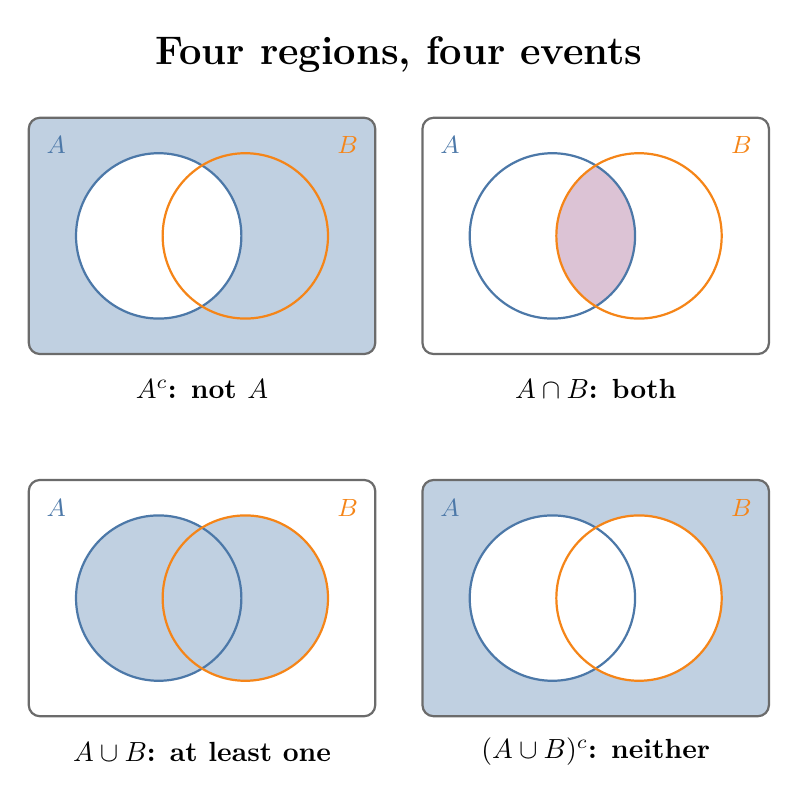
\begin{tikzpicture}[x=1cm, y=1cm]
  \node[title] at (2.5,2.3) {Four regions, four events};
  \panel{0}{0}{\fill[cblue!35] (-2.2,-1.5) rectangle (2.2,1.5); \fill[white] (-0.55,0) circle (1.05);}{$A^c$: not $A$}
  \panel{5}{0}{\clip (-0.55,0) circle (1.05); \fill[cpurple!45] (0.55,0) circle (1.05);}{$A \cap B$: both}
  \panel{0}{-4.6}{\fill[cblue!35] (-0.55,0) circle (1.05); \fill[cblue!35] (0.55,0) circle (1.05);}{$A \cup B$: at least one}
  \panel{5}{-4.6}{\fill[cblue!35] (-2.2,-1.5) rectangle (2.2,1.5); \fill[white] (-0.55,0) circle (1.05); \fill[white] (0.55,0) circle (1.05);}{$(A \cup B)^c$: neither}
\end{tikzpicture}
\end{document}
